

\section{User Module Sub-system}

The Users module is responsible for the management of NavUP's users. The system will consist of three types of users namely the admin,guest and normal users.The admin, who has more privileges than other users of the application, is mainly responsible for managing other registered users and managing information about venues and activities on campus.

\subsection{External Interfaces}
This section gives a detailed description of the system interfaces, hardware interfaces, software interfaces as well as communication interfaces.

	\subsubsection{System Interfaces}
		\begin{itemize}
			\item The user module will interface with any subsystem or module that wishes to access the data or               functions. 
		
		\end{itemize}
	\subsubsection{User Interfaces }
	\begin{itemize}

	\item The basic function of the user interface is to enable users to interact with the system.All the functions necessary to use the NavUP application are perfomed through the user interface. The user interface allows the user to login or register if they are first time users. 
 \end{itemize}
 
	\subsubsection{Hardware Interfaces }
	\begin{itemize}
	\item The will be a hardware interface with routers across campus in order to triangulate the position of the user on campus and this will require the hardware interface to interact with the Users module of the system. 
	\item The hardware interface also includes devices that users use to access the NavUP application 
	\end{itemize}

	\subsubsection{Software Interfaces } 
	The user module will communicate with the database in order to get the details of users for registration of updating user information, and also for saving locations etc. All the I/O interaction with the database.
	\subsubsection{Communication Interfaces } 

	The User module would be the core communicator in this system since every other subsystem is directly/indirectly related to user, so communication can be done through local message passing with internal events or via the abstract user management class, another means of implementation would be to consume the RESTful API within the system however this is very inefficient for an local internal event.



	
\subsection{Performance Requirements} %
User module should be able to perform under high CRUD operations,and have optimised methods to allow for faster execution and faster response times.


\subsection{Design Constraints}
\begin{itemize}

\item The speed at which NavUP can perform is constrained by the processing power and the  memory that is available on the device on which it runs.

\item The accuracy of the results profuced by functions such as determining the user's location, which are done by the GIS module through the Users module are constrained by the strength of the WIFI connection on campus.

\item This system’s ability to give updates and events to users through the Users module is constrained by the external management and maintenance which is performed by the administrator of the system.

\end{itemize}


\subsection{Software System Attributes} %
\subsubsection{Availability}
The user module should always be active since the majority of the application deals with the user module so having no down-time will be beneficial and required for the system to prevent crashes,
\subsubsection{Reliability}
The user module should make use of queuing for CRUD database operations, which most databases have and should be reliable since the database should be ACID compliant.

\subsubsection{Security}
Data within the user module should not have external classes accessing the information without being authenticated, user passwords and usernames should not be able to be accessed outside the scope of this module. Passwords should be encrypted using a strong encryption algorithm such as SHA-512 and should also support end-to-end encryption to guarantee more safer data transfer. The REST API should not be overexposed and have the necessary security implementations such as public/private key encryption, and should only accept authentic connections and prevent against DDOS.

\subsubsection{Auditability}
All CRUD operations within the user module should be logged for security and data integrity purposes.

\subsection{UML Diagrams}
\subsubsection{Class Diagram}
The class diagram of the user sub-system makes use of the template method design pattern so that if need be one can easily construct different types of users with minimal code modifications.

\begin{figure}[H]
	\centering
	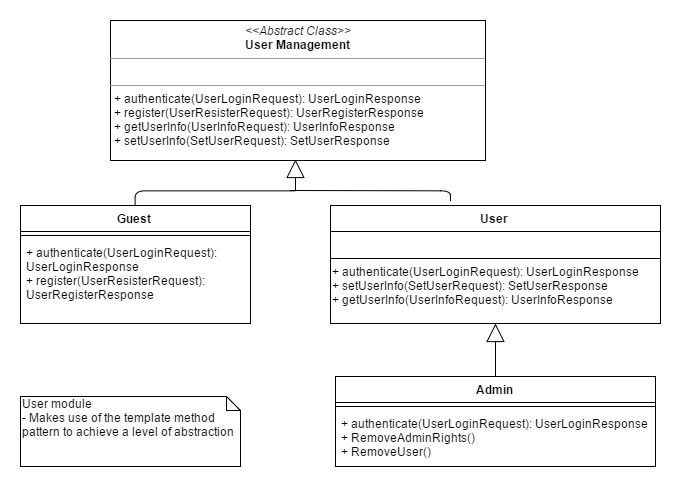
\includegraphics[width=0.7\textwidth]{user/img/UserClassDiagram.jpg}
	\caption{User Class Diagram}
\end{figure}



%\subsection{Deployment Diagram}
%
%\begin{figure}[H]
%%	\centering
%%	\includegraphics[width=\textwidth]{user/img/}
%%	\caption{}
%\end{figure}
%
%
\subsubsection{Activity Diagram}

\begin{figure}[H]
		\centering
		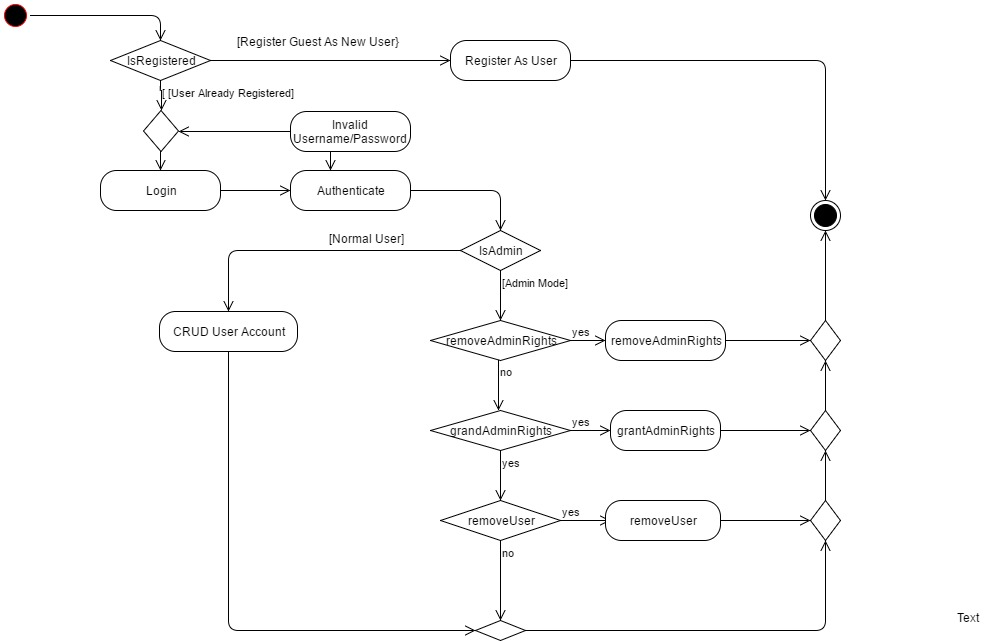
\includegraphics[width=\textwidth]{user/img/UserActivityDiagram.jpg}
		\caption{User Activity Diagram}
\end{figure}


\subsubsection{Sequence Diagram}
This diagram models time-ordered interaction behaviour between a user logging in and the interaction with the user subsystem.
\begin{figure}[H]
		\centering
		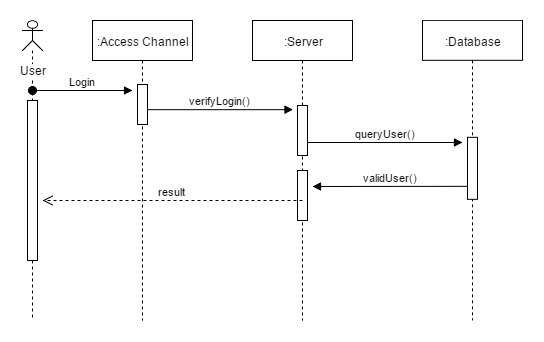
\includegraphics[width=0.7\textwidth]{user/img/UserSequence.jpg}
		\caption{User Login}
\end{figure}



\subsubsection{State Diagram}

\begin{figure}[H]
		\centering
		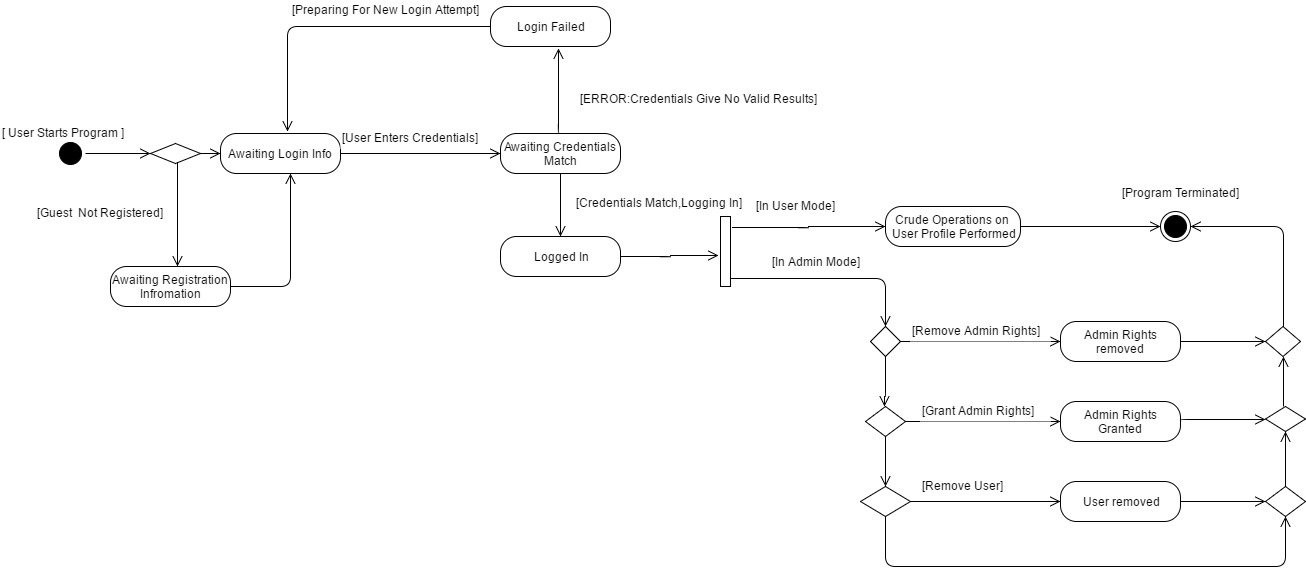
\includegraphics[width=\textwidth]{user/img/UserStateDiagram.jpg}
		\caption{User Login State Diagram}
\end{figure}




\subsubsection{Use Case Diagram}
This is a refined version of the use case diagram given in the Requirements Specification. It shows the functions of the subsystem as well as relationships of external entities or actors. This refined version also includes a detailed flow of use cases.
\begin{figure}[H]
		\centering
		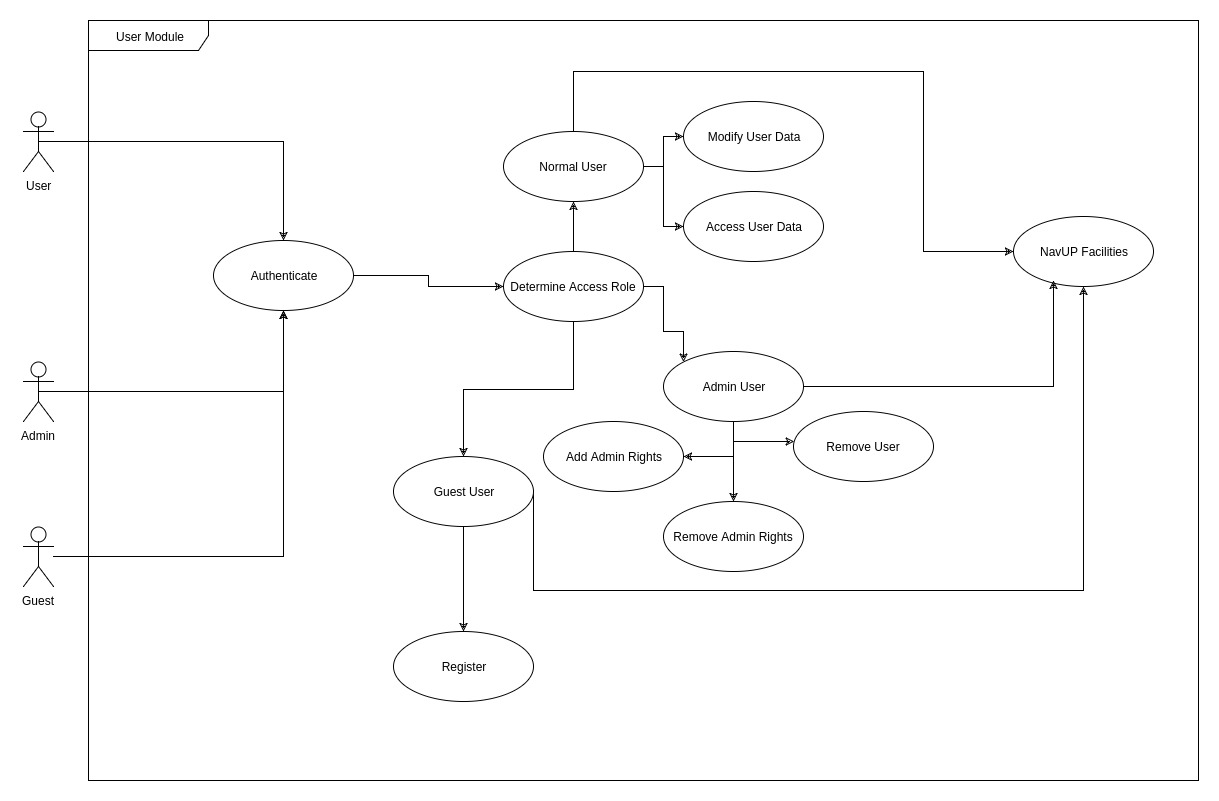
\includegraphics[width=0.7\textwidth]{user/img/UserUseCase.jpg}
		\caption{User Login with core functionality }
\end{figure}



